  %%%%%%%%%%%%%%%%%%%%%%%%%%%%%%%%%%%%%%%%%%%%%%%%%%%%%%%%%%%%%%%%%%%%%%
% LaTeX Example: Project Report

%%% Preamble
\documentclass[paper=a4, fontsize=11pt, abstract=on]{scrartcl}
\usepackage[T1]{fontenc}
\usepackage{fourier}
\usepackage{tabularx}
\usepackage[utf8]{inputenc}
\usepackage{hyperref}





\usepackage{listings}
\usepackage{color}

\definecolor{dkgreen}{rgb}{0,0.6,0}
\definecolor{gray}{rgb}{0.5,0.5,0.5}
\definecolor{mauve}{rgb}{0.58,0,0.82}
\lstset{frame=tb,
  language=[Visual]C++,
  aboveskip=3mm,
  belowskip=3mm,
  showstringspaces=false,
  columns=flexible,
  basicstyle={\small\ttfamily},
  numbers=none,
  numberstyle=\tiny\color{gray},
  keywordstyle=\color{blue},
  commentstyle=\color{dkgreen},
  stringstyle=\color{mauve},
  breaklines=true,
  breakatwhitespace=true,
  tabsize=3
}
\usepackage{graphicx}
\usepackage{caption}
\usepackage{subcaption}

\usepackage[english]{babel}															% English language/hyphenation
\usepackage[protrusion=true,expansion=true]{microtype}	
\usepackage{amsmath,amsfonts,amsthm} % Math packages

\usepackage{url}
%\usepackage[hang, small,labelfont=bf,up,textfont=it,up]{caption}


%%% Custom sectioning
\usepackage{sectsty}
\allsectionsfont{\normalfont\scshape}
\usepackage{float}
\usepackage{amsmath}
\usepackage{mathtools}
\usepackage{ragged2e}

\usepackage{nomencl}
\makenomenclature

%%% Custom headers/footers (fancyhdr package)
\usepackage{fancyhdr}
\pagestyle{fancyplain}
\fancyhead{}											% No page header
\fancyfoot[L]{}											% Empty 
\fancyfoot[C]{}											% Empty
\fancyfoot[R]{\thepage}									% Pagenumbering
\renewcommand{\headrulewidth}{0pt}			% Remove header underlines
\renewcommand{\footrulewidth}{0pt}				% Remove footer underlines
\setlength{\headheight}{13.6pt}
   \renewcommand*\abstractname{Summary}

%%% Equation and float numbering
\numberwithin{equation}{section}		% Equationnumbering: section.eq#
\numberwithin{figure}{section}			% Figurenumbering: section.fig#
\numberwithin{table}{section}				% Tablenumbering: section.tab#


%%% Maketitle metadata

\newcommand{\horrule}[1]{\rule{\linewidth}{#1}} 	% Horizontal rule

\title{
		%\vspace{-1in} 	
		\usefont{OT1}{bch}{b}{n}
		\normalfont \normalsize \textsc{} \\ [25pt]
		
\includegraphics[width=0.2\linewidth]{ubc.png} \\
		%
\includegraphics[width=0.4\linewidth]{tru}		
		\horrule{0.5pt} \\[0.2cm]
		\huge Term Project : Temperature Distribution inside Hydrogen Storage Tank \\
		\horrule{2pt} \\[0.005cm]
}
\author{
		\normalfont 								\normalsize
        Jerin Roberts\\[-5pt]		\normalsize
        \today
}
\date{}




%%% Begin document
\begin{document}
\maketitle
\begin{center}
\begin{tabular}{l r}


Supervisor: & Dr. Patrick Kirchen  \\ % supervisor
Locations: & University of British Columbia


\end{tabular}
\end{center}
\newpage
\begin{abstract}
  need abstract
\end{abstract}


\newpage
\tableofcontents
\listoffigures
\listoftables
\newpage
\lstset{language=[Visual]C++}

\mbox{}% need to run this: makeindex TermProject.nlo -s nomencl.ist -o TermProject.nls

 
\nomenclature{$\rho$}{Density $kg/m^3$}
\nomenclature{$T$}{Temperature $K$}
\nomenclature{$P$}{Specific Pressure}
\nomenclature{$V$}{Volume $m^3$}
\nomenclature{$p$}{Pressure $MPa$}
\nomenclature{$\mu_{JT}$}{Joule-Thompson Coefficient}
\nomenclature{$C_P$}{Pressure Coefficient}
\nomenclature{$R$}{Ideal gas constant}
\nomenclature{$v$}{Velocity $m/s$}
\nomenclature{$m$}{Mass $kg$}



 
\printnomenclature

\newpage

\section{Introduction}


A Hydrogen has long been in consideration as of the top ecological replacements to gasoline fueled internal combustion engines. Having water as the byproduct burning pure hydrogen produces zero emissions. Although finding pure hydrogen is rare in the earths crust it can be access from many other abundant chemicals via electrolysis or reforming methods. Having a high specific energy density of 39 $kWh/kg$ and only water production as emissions hydrogen fuel could provide an effective alternative. However gaseous hydrogen has a low volumetric energy density 3.5 $kWh/m^3$ at standard temperatures  and conditions making it difficult to store effectively and efficiently. 

\section{Background}
\subsection{Storage Sates}
The two prevailing states for storing are in compressed gaseous and cryogenic liquid states, however both methods still present a number technical challenges that need to be overcome before the technology can be successfully implemented into modern transportation infrastructures. 

At first glance the liquid form seems to be the ideal solution. Having a very high specific and volumetric energy density it can expanded into a gas easily for combustion. The two challenges that are faced with liquid hydrogen are the process for obtaining a liquid state and the measures for preserving that state. Acquiring liquid hydrogen requires various throttling and cool down methods to bring the hydrogen to a low enough temperatures to liquefy. To exist as a liquid the H2 must be cooled below hydrogen's critical point of 33 K and in order to maintain a fully liquid state without boiling at atmospheric pressure needs to be cooled further to 20.28 K. Maintaining the temperatures requires cryogenic storage technology such as thermally insulated containers and requires special handling procedures common to all cryogenic fuels. However even with thermally insulated containers it is difficult to keep such a low temperature, and the hydrogen will gradually leak away usually at a rate of about 1\% per day. These technical challenges will require additional expensive and complex systems, which makes liquid hydrogen less ideal as an energy carrier.

\begin{figure}[H]
        
        \begin{subfigure}[H]{0.45\textwidth}
        \centering
                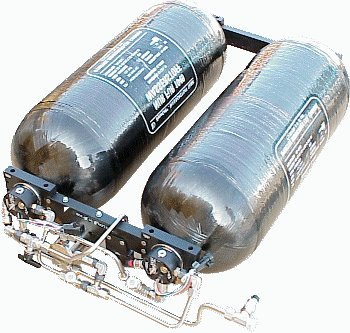
\includegraphics[height = 4.5cm]{tank1}
                \caption{}				
        \end{subfigure}%
       ~~~~~
        \begin{subfigure}[h]{0.45\textwidth}
        \centering
                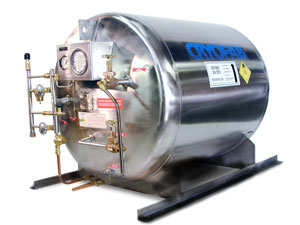
\includegraphics[height = 4.5cm]{cry}
                \caption{}
                
        \end{subfigure}
        ~~~~~
        \caption{Compressed Gaseous system (a) vs Liquid hydrogen system (b)}
        \label{results}
\end{figure}

The technical challenges of bringing compressed hydrogen fueling systems to market lie in the associated storage and re-fueling systems. Specifically using gaseous hydrogen requires significant compression of the gas in order to obtain a viable volumetric energy density +350 bar. In order to adopt these pressures while conforming to safety constraints special high pressure vessels are required.  Type 3 and 4 are typically used for high compression systems 350-700 bar. At these higher pressures the volumetric energy density of hydrogen is found to be ~1500 $kWh/m^3$, which is significantly higher than hydrogen under normal standard conditions, however still does not compare to gasoline fuels which are around 9000 $kWh/m^3$.However this is offset by hydrogen's high specific energy density and zero emissions. Another technical aspect lies in the behavior of hydrogen under fast filling conditions. In order for the technology to be successful it needs to be as good or better than current technologies. This means the refueling process needs to be as fast or faster than typical gasoline pump times. Compressing or transferring hydrogen into vehicle tanks at these pressures produces significant heat and ultimately limits the attainable fill rates. Additionally the quality of the fill is related to the temperature gain of the hydrogen during transfers. As the hydrogen cools the pressure decreases subsequently causing the tank to become partially filled.  

\subsection{Tank Types for Gaseous Hydrogen}
Pressurized Gaseous Hydrogen can be stored on board vehicles using compressed gas method. This method of storage is the simplest and most cost effective technology for hydrogen storage as it requires little supporting systems for maintenance. The gas undergoes compression at a fueling station and dispensed into the on-board tank of the vehicle. There exists 4 types of tanks used to safely store compressed hydrogen. These types are labeled as type 1,2,3 and 4. Figure \ref{tank} displays a simple diagram of a type 4 high pressure tank used for hydrogen storage.


\begin{figure}[H]
\centering
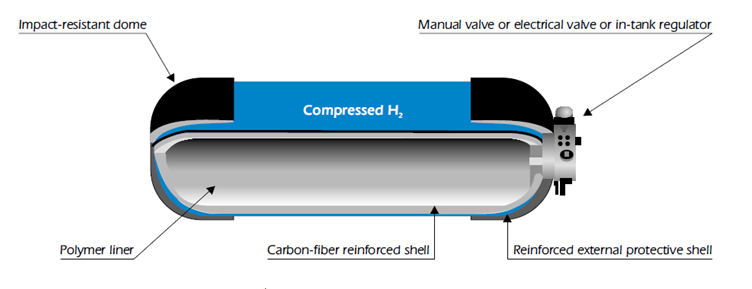
\includegraphics[width=0.8\linewidth]{tank2}
\caption{Diagram of a hydrogen type 4 storage system}
\label{tank}
\end{figure}

 Type 1 is a basic metal tank while type is a metal tank with a fiber wrapping. These are typical of lower pressure systems (sub 300 bar) and have significantly lower performance factors due to their relatively high weight and lower capacities. Type 3 tank is a metal liner with full reinforcing fiber wrapping, while type 4 is the same as type 3 but instead with a polymer liner. These tanks are described as having a very high performance factor, attributed to their design which maximizes volume and pressure while reducing tank construction weight.  Currently, majority of demonstration and prototype vehicles employ cylinders capable of storing hydrogen up to 350 bar, while new lightweight composite type 3 and type 4 gas cylinders have been developed to withstand pressures up to 800 bar. Due to these new advances new data is required to understand the challenges with filling these tank at reasonable rates.



\subsection{Fueling}
Generally the tanks design for fuel storage will not contain any pumps or systems to maintain pressure. Therefore the hydrogen will need to be filled to rated pressure and capacity from an external source. Much like petrol stations hydrogen can be obtain through dispensers and stations in which high-pressure gas is moved from a large station reservoir into the smaller vehicle cylinder. Figure \ref{station} displays the general layout for a hydrogen dispenser. Generally the main storage tanks (supply source) will be keep the hydrogen at a lower pressure which will be compressed into buffer tanks when required. The buffer tanks allow the compressed hydrogen to remain cool and provide varying levels of pressure for efficient filling. To avoid overheating hydrogen the buffer tanks will be accessed in acceding orders of pressure. This stepping methods reduces the heat and improves efficiency of the dispenser. The rate of gas transfer and safety of filling are controlled by the station dispenser. As the temperature of the gas cools to ambient the pressure also decreases such that the cylinder is no longer filled to design capacity. This is generally termed as under filling. In order to avoid this situation cylinders are filled to rated mass, which due to the temperature increase results in the cylinder being filled beyond the rated service pressure. 

\begin{figure}[H]
\centering
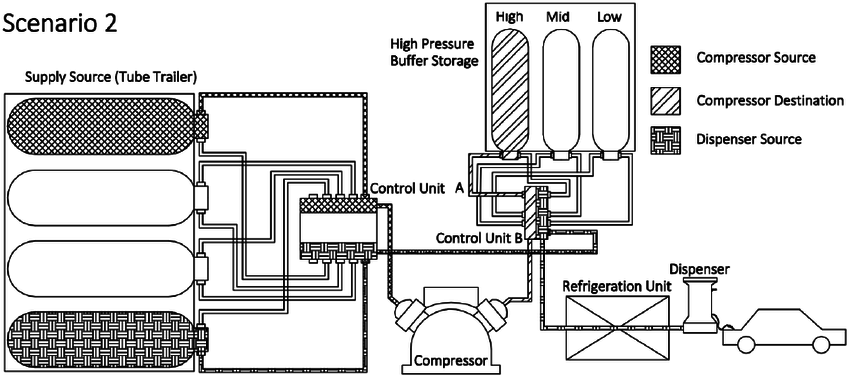
\includegraphics[width=0.8\linewidth]{station}
\caption{Simple Diagram of a hydrogen refueling station}
\label{station}
\end{figure}


 The goal of the dispenser is to fill the cylinder to the rated mass of gas without exceeding the pressure and temperature limits of the cylinder. In order to complete the filling, the dispenser must employ a method for calculating the mass of gas present inside the cylinder. Generally a flow-rate measurement and a pressure measurement will be used to estimate the total mass transferred during the fill. The metering systems for safety will need to know the values of pressure and temperature to a high accuracy and typically will have some way of receiving data from built in sensors on the vehicle tank. In order for this to be possible the temperature and pressure of the gas inside the tank need to be well characterized. With this known the location of the pressure and temperature sensors can be place appropriately as too best represent the state of the gas through out the entire tank. When the sensors are well placed they will best represent accurately the mass of hydrogen moved and allow the dispenser to know when to terminate.



\section{Theory}

\subsection{Gas Heating}
During the fill process is a significant increase in gas temperature can be seen. The temperature rise during filling is the result of the combination of two dominating phenomena; Joule-Thompson effect and standard gas compression. In thermodynamics the Joule-Thomson effect is a process in which a gas or liquid is forced through a valve or porous plug and as a result experience a temperature change. Generally most gases at room temperature cool upon expansion by the Joule-Thomson process. However a couple gases like hydrogen, helium and neon will heat when throttled. This is because their Joule-Thomson coefficient is negative corresponding to a heating effect during a free expansion. The coefficient is a function of temperature and pressure under isenthalpic conditions as shown in equation \ref{jte}


\begin{figure}[H]
\centering
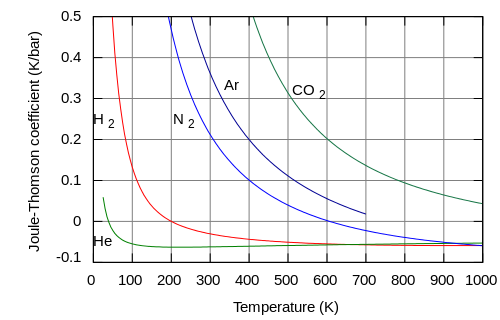
\includegraphics[width=0.5\linewidth]{jt}
\caption{Joule-Thompson Coefficients for different gases}
\label{jt}
\end{figure}

Similarly gas and liquids with positive coefficients will be cooled. It should be noted this coefficient is dependent on the state of the gas and therefore exists a point were the sign can flip which is known as the inversion temperature. Hydrogen has a negative Joule-Thomson coefficient at the temperatures and pressures of filling. Therefore when the gas experiences an isenthalpic expansion from the high-pressure tank through the dispenser throttling device into the low-pressure cylinder its temperature will increase. It is important to note that the isenthalpic expansion occurs within the dispenser which results in a higher gas temperature entering the cylinder. Figure \ref{jt} displays how the effect of temperature on the Joule-Thompson coefficient of a gas.

\begin{equation}
\label{ideal}
p=\frac{RT}{V_m-b}-\frac{a}{\sqrt{T}V_m(V_m+b)}
\end{equation}

\begin{equation}
\label{jte}
\mu_{JT} = \Bigg(\frac{\partial T}{\partial P}\Bigg)_H
\end{equation}

The second phenomenon that causes a temperature rise during filling is the actual compression of the gas inside the cylinder. At the start of filling the gas is compressed by the introduction of the higher-pressure gas from the fueling station. This is repeated throughout the fill as the new gas moving into the cylinder compresses the gas currently in the cylinder. When a gas is compressed generally it will experience a temperature increase as is seen in the Redlich-Kwong model equation \ref{ideal} for an real gas. The increase in temperature is often referred to as the heat of compression \cite{dick}. 



\subsection{Modelling}
The main problem with measuring the temperature distribution in all aspects of the tank is the requirement for a discrete measurement at every spacial point inside. This in practice is nearly impossible for both reasons of cost and invasive action of the process. Modeling provide a relatively cheap alternative to measurements and can very power when used in parallel with experimental measurements. As part of the characterization of this process a CFD model will be built and validated using the ANSYS workbench and Fluent. Fluent is a Computation Fluid Dynamics program which uses primarily finite volume methods to calculate numerical solutions to fluid domain problems. In order to describe the problem a spacial domain will need to be define. Fluent does this by generating a geometrical mesh to match the exact dimensions of the tank and fluid domain volume used for the test. Once this has been generated a user defined library will have to be added as fluent does not include default libraries for real gas calculations for hydrogen gas. A Redlich-Kwong real gas model will be implement via a user define function (UDF). A UDF can also be created and used to simulate time depend boundary conditions. The Boundary and initial conditions will have to be experimentally recorded along with the data for a fast fill run. The model will use the experimental conditions as initial parameters and time varying measurements like pressure and inlet temperature for time dependent boundary and inflow conditions. 
\begin{figure}[H]
\centering
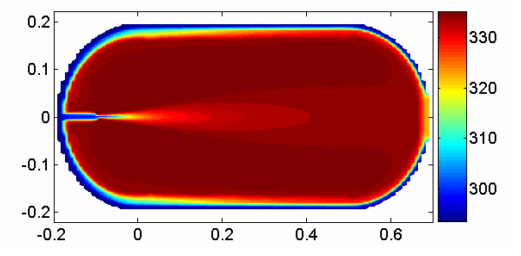
\includegraphics[width=0.8\linewidth]{mod1}
\caption{Displays model of temperature distribution inside 350bar tank \cite{dick}}
\label{comp}
\end{figure}
Once all the necessary parameters have been set for the model its results will be compared against the actual experimental results. If the average deviation between the model and experiment is below a certain standard the model can be used to accurately predict temperature for all points through-out the tank. If the error is too large the underlying physics of the model will have to be re-evaluated until acceptable error is reached. Figure \ref{mod} displays an example of a model evaluated for temperature during a 350 bar tank fill.

\subsection{Temperature}
The final results of the model is a temperature distribution inside the tank, therefore temperature will need to be measured at key locations inside the tank to validate model. Temperature is hard to measure directly and its usually easy to measure another phenomenon closely associated with it. A thermocouple is an electrical device consisting of two or more conductors of differing material which in turn form electrical junctions at differing temperatures.  At the atomic scale, an applied temperature gradient across a conductor causes charge carriers in the material to diffuse from the hot side to the cold side. Therefore the device produces a temperature-dependent voltage as a result of the thermoelectric effect. This voltage can be interpreted and calibrated to measure temperature. A thermocouple is displayed in figure \ref{therm}

\begin{figure}[H]
\centering
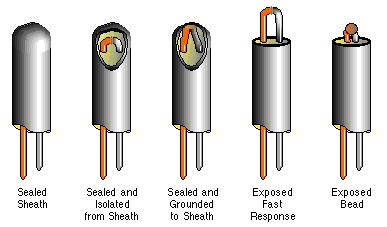
\includegraphics[width=0.5\linewidth]{thermom}
\caption{Different thermocoupler ends}
\label{therm}
\end{figure}

\subsection{Mechanical Force}
Pressure is another property that is hard to directly measure. Fortunately pressure can apply a mechanical force to an object causing displacement over time which is something relatively easy to measure directly. Diaphragm transducers use a diaphragm to make a relative measurement between two pressure sources. When the sources are of equal pressure then equal force is applied to both side of diaphragm keeping it stationary and undeformed. If one source were greater than the older the diagram will have unbalance forces acting on it causing it to deform slightly. This deformation can be measured using strain gauges or capacitance sensors and thus provides a means of turning mechanic force into an electric signal which is directly proportional to pressure.

\begin{figure}[H]
\centering
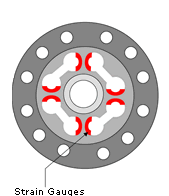
\includegraphics[width=0.3\linewidth]{loads}
\caption{Cross section of pancake style load cell displaying locations of strain gauges}
\label{loads}
\end{figure}


Strain gauge load cells convert the load acting on them into electrical signals. Much like in the pressure transducer the strain gauges themselves are bonded onto a beam or structural support that deforms when force is applied. Generally a load cell will contain a compression orientated and a tension orientated strain gauge. When weight is applied to the load cell, some strain gauges compress decreasing their resistances while simultaneously the tension ones stretch increasing their resistances. The difference in resistance causes different currents to run through each, thus creating a potential difference that can be measured. The gauges are often mounted in a differential bridge to enhance the accuracy of the measurement. Figure \ref{loads} displays the cross section of a pancake style load cell.



\section{Methodology}

For this project the requirements are to map out the temperature distribution inside a hydrogen tank during a fast fill to provide a solid measure of average temperature and to find a suitable temperature location that best represents such. A combination of both modeling and experimental studies will be used to determine such point. Modeling given its valid should show the ideal location for temperature measurement. Therefore an experimental apparatus is created to help validate the thermodynamic model produced. In order to validate the model measurements of temperature at keys locations, pressure, and mass flow rate need to be recorded accurately during the entire fast fill cycle. The constraints for the experimental validation are displayed in table \ref{con}

\begin{table}[H]
\begin{center}
    \begin{tabular}{ | p{0.15\linewidth} | p{0.45\linewidth} | p{0.35\linewidth} |}
 \hline  
     \RaggedRight \textbf{Constraint}
    &\RaggedRight \textbf{Description}
    &\RaggedRight \textbf{Solution}
    \\ \hline  
           \RaggedRight 2D $\triangle T$
    &\RaggedRight Map out 2D temperature distribution within tank during transient fill
    &\RaggedRight Array of sensors with exact locations known inside tank
    \\ \hline 
           \RaggedRight $\triangle m$
    &\RaggedRight Measure accurately mass before fill, end of fill, and after cool down
    &\RaggedRight Use high accuracy scale
    \\ \hline 
           \RaggedRight $\triangle P$
    &\RaggedRight Measure Transient pressure during fast fill and cool down
    &\RaggedRight Pressure Sensor at inlet and far end of tank
    \\ \hline 
    \RaggedRight Semi-Portable
    &\RaggedRight System needs to be semi portable as system will need to be transported to hydrogen dispenser 
    &\RaggedRight Design experimental apparatus and DAQ to fit on transportable push trolley 
    \\ \hline 
    \RaggedRight Standard Tank
    &\RaggedRight No modifications to tank are permitted 
    &\RaggedRight Collapsible sensor array to be inserted and expanded inside tank
    \\ \hline 
    \RaggedRight Adhere to SAEJ2601
    &\RaggedRight Adhere to standards and procedures for the fast filling of hydrogen type 4 tanks 
    &\RaggedRight Have 1-2 sensors report data to dispenser
    \\ \hline 
    \RaggedRight Non-Invasive
    &\RaggedRight Reduce the effects of the measurement on the internal process
    &\RaggedRight Use insulating materials for sensor support, minimize size and fluid obstruction of array.
    \\ \hline 
    \end{tabular}
\end{center} 
\caption{Constraints for experimental validation}
\label{con} 
\end{table}


\subsection{Experimental Setup}
The overview of the proposed experimental setup is displayed in figure \ref{exp}
A tank will be mount to a trolley with a load cell buffer in between, which wll allow for mass change measurements. The tank will be a type 4 700 bar rated capacity tank specialized for hydrogen storage. The cylinder is manufactured by Luxfer Industries (part\# M030H) which has an internal volume that translates into 1.12 kg of stored hydrogen at a pressure of 700 bar (69.95MPa) with a temperature of 15 °C (288 K). The entire tank including fuel will weigh approximately 60 pounds. The diagram of the tank to be used in the experiment is displayed in figure \ref{tschem}. 


\begin{figure}[H]
\centering
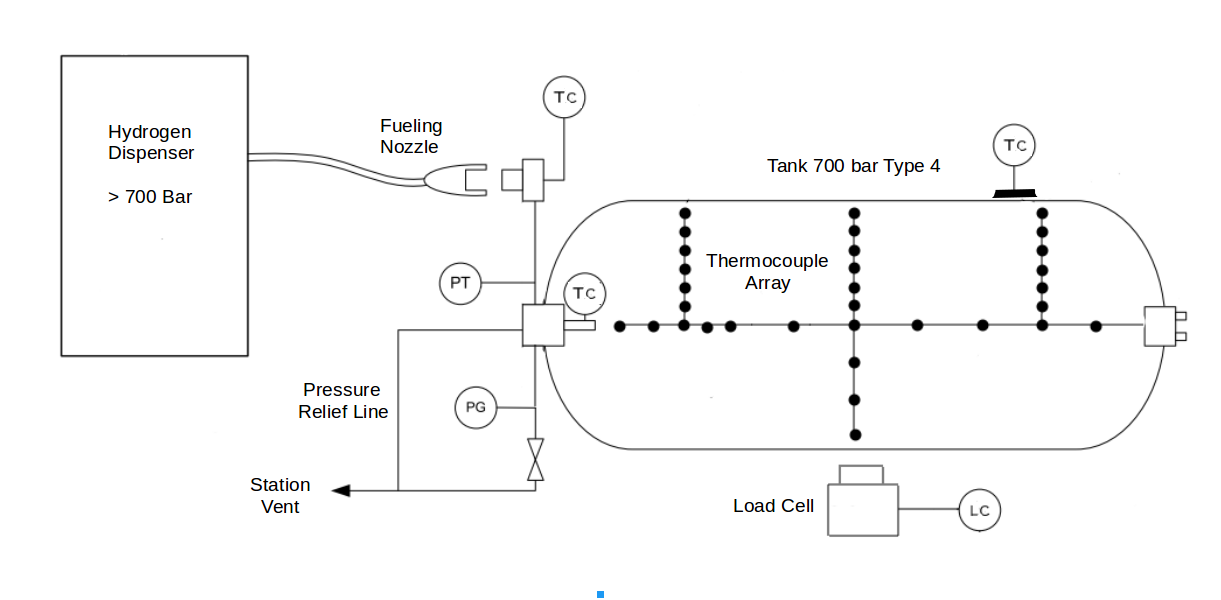
\includegraphics[width=0.95\linewidth]{schem2}
\caption{Diagram of the proposed experimental setup}
\label{exp}
\end{figure}





The tank contains two openings each with a 2" threaded insert. One side will be used for attaching the filling equipment while the other for the array matrix. The filling side of the cylinder will be equipped with either an off the shelf or custom internal tank valve block assembly. The assembly will house a solenoid or pneumatic valve, a manual shutoff valve, a pressure relief device, and a Bourbon reference gauge. Likely an off the shelve block will also include a thermistor mounted internally for dispenser communication. The opposite end of the cylinder will have a custom built block with support bracket for the array as well as a sealed conduit for the thermocouple wire management.

\begin{figure}[H]
\centering
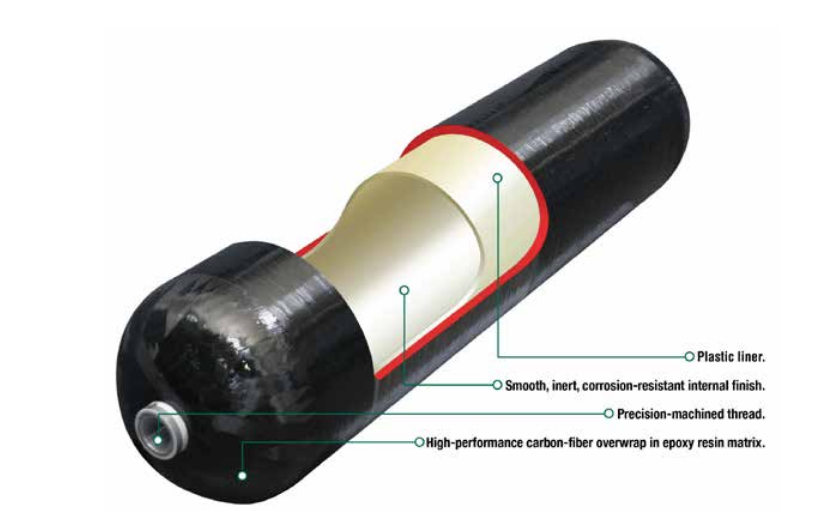
\includegraphics[width=0.6\linewidth]{tschem}
\caption{Examples of Drag coefficient as a function of Reynolds number for common objects}
\label{tschem}
\end{figure}


\subsection{DAQ} 



The data acquisition system was chosen with accuracy and precision in mind while maintaining the ability to remain semi portable. The large thermocouple array requires at least 32 channels for transient measurements along with another 4-6 additional measurements. For these reasons a National Instruments System Was selected. Table \ref{daq} displays the devices used for collecting and managing sensor data. The Heart of the system is the eDAQ-9174 which serves as the step between the ADC and the software. It runs a user define program compile from labview for gathering data from all modules and organizing it relative to a time stamp or sample count. All of this is then compressed and communicated to a local system running labview via a simple USB interface for storage. This 9174 contains 3 card slots for running different ADC/modules simultaneously. This provides a great tool for collecting and organizing all the time dependent data and eliminates the need for complex syncing schemes. Two types of ADC's have been selected to run with the experiment. 


\begin{figure}[H]
\centering
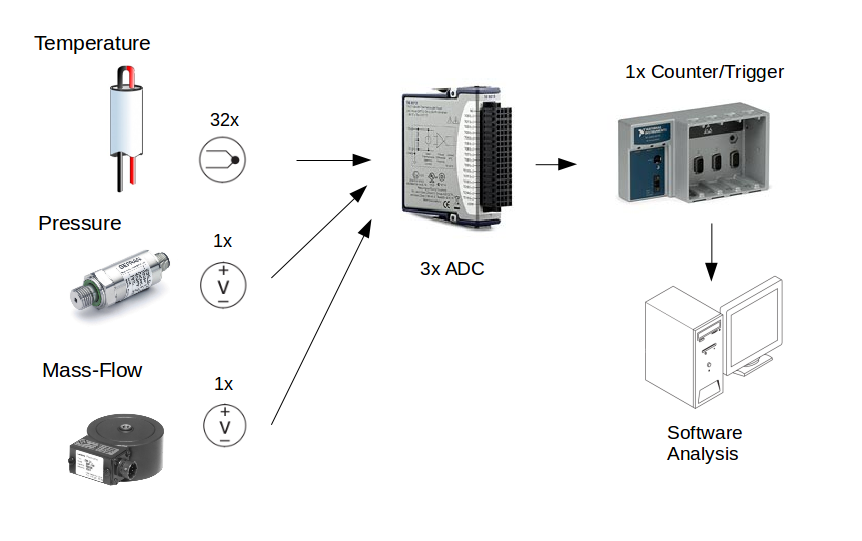
\includegraphics[width=0.8\linewidth]{sch}
\caption{Examples of Drag coefficient as a function of Reynolds number for common objects}
\label{daqd}
\end{figure}


The NI 9213 ADC is a module optimized for thermocouple measurement. Each module features a $\pm78$ input with 16 channels and an internal cold-junction compensation sensor. The card runs a 24bit ADC at a 100kS/s sampling rate making it perfect for large transient data collections. For the pressure and load cell data aquisition a 4ch high speed 16 bit ADC was selected. The system features 0-10V and $\pm$5V input range making it easy to couple most devices with DC output. 


Figure \ref{daqd} displays the general layout of the DAQ system.

 

\begin{table}[H]
\begin{center}
    \begin{tabular}{ | p{0.20\linewidth} | p{0.20\linewidth} | p{0.45\linewidth} |}
 \hline  
     \RaggedRight \textbf{Device}
    &\RaggedRight \textbf{Description}
    &\RaggedRight \textbf{Specifications}
    \\ \hline  
           \RaggedRight 2x NI 9213
    &\RaggedRight Thermocouple ADC
    &\RaggedRight -16ch 24 bit ADC \newline -$\pm$78.125mV input range \newline - 78 S/s sampling rate \newline -accuracy with type T $\pm 0.02^{\circ}$C
    \\ \hline 
           \RaggedRight 1x NI 9215 
    &\RaggedRight Transient Relative Pressure Measurment
    &\RaggedRight -4ch 16 bit ADC \newline - $\pm$10V input range \newline - 100 kS/s sample rate \newline - $\leq 0.2\%$ error (calibrated)
    \\ \hline 
           \RaggedRight Honeywell 3397 Load Cell
    &\RaggedRight $\triangle m$ measurement for fast fill and cool down
    &\RaggedRight  
    \\ \hline 
    \end{tabular}
\end{center} 
\caption{Constraints for experimental validation}
\label{daq} 
\end{table}




\subsection{Temperature}
The spacial distribution of temperature is this case is the ost challenging aspect of the measurement system. The system needs to attain a fairly high level of accuracy while maintaining sensitivity all while needing to fit through a 2" hole. For these reason thermocouples were chosen as the most suitable sensor. 

\begin{figure}[H]
\centering
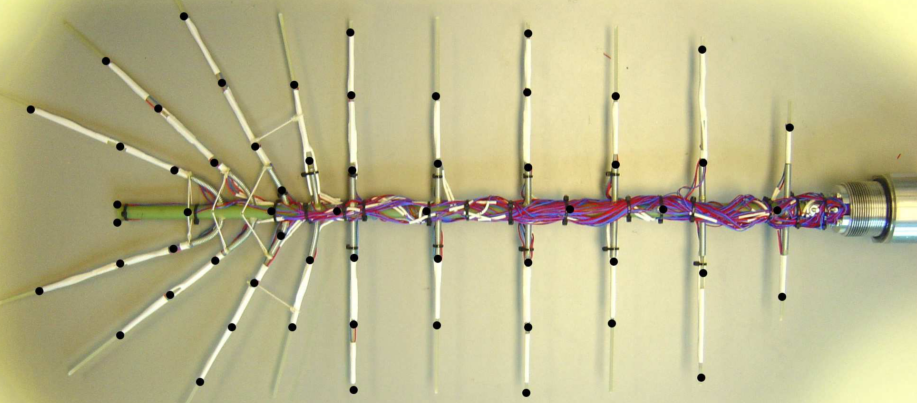
\includegraphics[width=1.0\linewidth]{array}
\caption{Example of a collapsible thermocoupler array to be inserted into tank \cite{dick}}
\label{array}
\end{figure} 



 Thermocouples are self powered and will not require a power supply which due to the shear number of sensors used in the array is a huge advantage. Running an extra line for every device for excitation would add a lot of complexity to the sealed conduit as well as taking up additional volume inside the cylinder. Another advantage of thermocouplers is there sensitivity to transient events. During the fast fill process a dynamic process is expect therefore a device with transient capabilities is needed. The main limitation with thermocouples however can be accuracy in the respect that system errors of less than one degree Celsius (°C) can be difficult to achieve. Due to there transient nature however the error can be mitigated by running an averaging scheme at high refresh rates. Thermocouples come in many varities and are characterized by the materials used as the conductors. For this experiment a T type thermocouple was selected to be used in the internal array. The T type contains copper-constantan junction which makes it suitable for a large range of measurements. Type T is non-reactive with hydrogen and has a fast response making it ideal for this application. The complete device specifications are found in table \ref{sens}. An collapsible structure will be fabricated of insulating materials such as ABS or PLA in order to strategically set the thermocouplers to a known position. The structure will be collapse before inserted and will be erected either from external intervention or automatically by a rubber elastic spring system. Figure \ref{array} displays an example of a collapsible array of thermocouples used in similar studies \cite{dick}.
 
\begin{table}[H]
\begin{center}
    \begin{tabular}{ | p{0.15\linewidth} | p{0.30\linewidth} | p{0.25\linewidth} |p{0.20\linewidth} |}
 \hline  
     \RaggedRight \textbf{Sensor}
    &\RaggedRight \textbf{Specifications}
    &\RaggedRight \textbf{Input/Output}
        &\RaggedRight \textbf{Calibration}
    \\ \hline  
           \RaggedRight Type T\newline Thermocouple
    &\RaggedRight -Exposed 0.008mm End \newline - Special Grade\newline - $\pm 0.5^{\circ}$C or $0.4 \%$ accuracy \newline - $\tau = 0.15$ s response
     &\RaggedRight -No excitation \newline -Differential Output \newline $\pm$78 mV
     &\RaggedRight - NIST rational polynomial method \newline - Cold Junction Sensor
    \\ \hline 
           \RaggedRight Gefran KS Pressure Transducer
    &\RaggedRight - 0-100 MPa range  \newline -$\pm 0.5\%$ accuracy FS \newline - $10^{-3}$ s $10-90\%$ response
     &\RaggedRight - 0-10V output \newline - 30Vdc excitation
     &\RaggedRight Calibration Curve
    \\ \hline 
           \RaggedRight Honeywell 3397 Load Cell
    &\RaggedRight  - 0-200lb range \newline - 2mV/V $\pm 0.25\%$ accuracy \newline - 1.0s response 10-90\%
     &\RaggedRight - With Universal Inline Amplifier $\pm$10Vdc \newline - 30Vdc excitation
     &\RaggedRight Experimental Calibration Curve
    \\ \hline 
    \end{tabular}
\end{center} 
\caption{Constraints for experimental validation}
\label{sens} 
\end{table}

In addition to the array there will be discrete temperature measurements made at key locations around the experiment. The inlet temperature of the incoming hydrogen will be measured using both a Type T thermocouple and a thermistor provided by the selected block valve. The thermistor will be used as the input for the dispenser and its value will not be logged using the DAQ and instead will be noted for consistency. The thermocouplers will be calibrated and referenced using the rational polynomial function approximation for Type T thermocouples. Using a least squares curve fitting procedure we will fit the National Institute of Standards and Technology (NIST) type T thermocouple data with a rational function.

\subsection{Pressure}
The pressure for the experiment will be measured at the inlet of the tank. Again the sensor needs to  be able to cope with high pressures and temperature fluctuations while maintaining accuracy and response. For this reasons a diaphragm transducer sensor was selected. For this experiment The Gefran KS series pressure transducer was selected which uses a capacitance film on a stainless steel diaphragm. A capacitance type sensor was selected for its robust construction, relative low dependence on temperature and its suitability for most transient processes. The sensor however requires an external excitation, but fortunately just one sensor is required and is access externally and therefore is not a huge issue. The specifications of the sensor are displayed in table \ref{sens}

\begin{figure}[H]
        
        \begin{subfigure}[H]{0.30\textwidth}
        \centering
                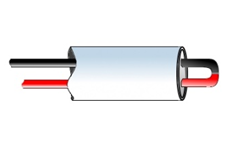
\includegraphics[height = 2.5cm]{Therm}
                \caption{}				
        \end{subfigure}%
       ~~~~~
        \begin{subfigure}[h]{0.30\textwidth}
        \centering
                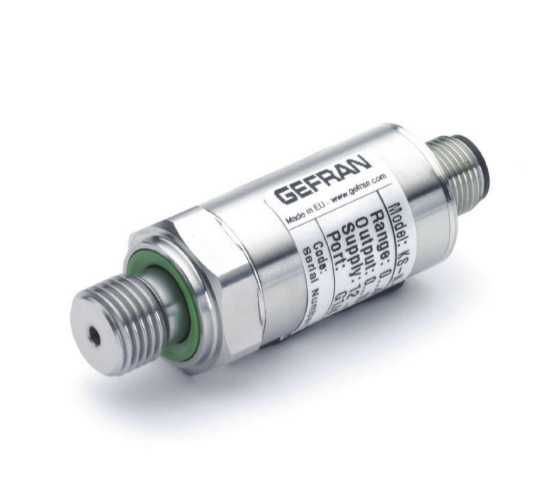
\includegraphics[height = 2.5cm]{press}
                \caption{}
                
        \end{subfigure}
        ~~~~~
        \begin{subfigure}[h]{0.30\textwidth}
        \centering
                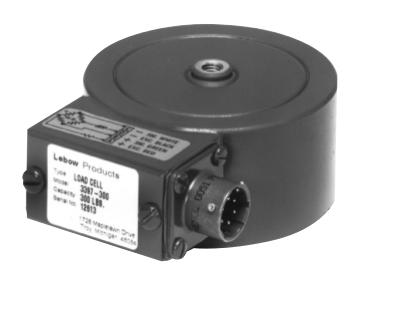
\includegraphics[height = 2.5cm]{load}
                \caption{}
                
        \end{subfigure}
        ~~~~~
        \caption{Displays the sensors selected for experiment: Type T thermocouple (a) GEFRAN pressure Transducer (b) and a Honeywell load cell (c)}
        \label{results}
\end{figure}
The pressure transducer will be mounted using standard practices such as welded nipple or tapped 'T' section. This measurement can skewed because of the pressure gradient that exists between the buffer tank in the dispenser and the vehicle side tank. Therefore its paramount that the pressure sensor be mounted as close to the tank inlet as possible as to best represent the pressure inside the tank. Because this is a relative measurement the sensor cannot be mounted internally as its needs exposure to the outside ambient pressure. A barometer will be used to measure the ambient temperature and pressure conditions.


\subsection{Mass}
The amount of hydrogen fuel moved into the tank will be measured using a simple load cell method. The load cell will be used to measure the change of mass of the tank during the fast fill and cool down period. The load cell method has some advantages and disadvantages versus a flow meter. Some of the advantages include its simplicity, relative low expense and its accuracy in comparison to flow meter methods. Additionally the load cell will be mounted externally from the tank and therefore will not be exposed to temperature fluctuations that could induce inaccuracies. However standard load cells can have a slow response which may lead to error describing the mass relative to time. One would have to make adjustments in order to match the data correctly. Fortunately the initial and final measurements for this process are the minimum that are required for model validation as the model uses pre-determined flow-rates.  Therefore measurements can be made at a much slower rate as we're not as concerned as much with the instantaneous rate of change but rather the overall rate of change. For these reasons employing a load cell is more effective method. A Honeywell Model 3397 load cell was selected for mass change measurements and its specifications are displayed in table \ref{sens}. It was be run with a linear amplifier circuit in order to convert its AC output to a DC 0-10V range making it easy to couple with standard DAQ systems. The load cell system will be calibrated by adding known mass and generating a calibration curve.
\subsection{Uncertainty}

\subsection{Procedure}
Once the experimental apparatus has been tested and all sensors properly connected and calibrated the apparatus will be taken to a dispensing facility. The Thermocoupler array will be inserted and properly erected with locations of a sensors measured and recorded using a precision ruler. The array will be run in different configurations to effective map out the behavior of the gas for a large region inside the tank. Once properly set the internal valve block assembly will be attached and the tank purged with nitrogen to avoid explosion hazards. The system will then be connected to hydrogen dispenser and re-purged this time with hydrogen. The dispenser will require input from an internal thermister built into the block value. All excess and vented gas will be directed to the station/dispenser vent. After ensuring all air and then nitrogen have been removed from the system the tank will be filled to 50 Bar and left to stabilize. Once stabilized all initial data will be recorded; initial tank mass, initial temperature, ambient references and selected ramp rates. The DAQ system will begin recording ensuring stable values. The fill will then be initiated as per SAEJ2601 standards for fast filling. Its likely due to the time requirements and expense of the hydrogen gas only one ideal ramp rate will be selected and studied. Pressure and Temperature with be sampled at 20S/s and averaged at 0.5 second intervals while the mass and ambient sensors @ 1S/s during Fast fill. The fill will either be halted when the pressure reaches the rated capacity for the tank (700Bar) or a maximum temperature of 80$\circ$C is reached for the internal block valve thermister. The tank will then be left to cool. Data will be recorded until temperature has stabilized at ambient at which point the final conditions will be recorded ending the run. The gas will be vented back down to 50 Bar and allowed to re-stabilized so that another run can be taken. This process will be repeated 5 times for each array arrangement for up to 10 different arrangements. To ensure continuity between measurements several sensors in the array will remain in the same positions for every measurement. Table \ref{pro} summarizes the steps for the experimental procedure.


\begin{table}[H]
\begin{center}
    \begin{tabular}{ | p{1.00\linewidth} |}
 \hline  
    \begin{itemize}
\item Transport Calibrated Apparatus to Dispensing site
\item Purge Tank and Set Pressure to 50 Bar
\item Allow Temperature/Pressure to Stabilize 
\item Record Initial Conditions
\item Apply Required Ramp Rate
\item Measure P, T @ 10S/s  m @ 1S/s during Fast fill
\item Measure P, T @ 10S/s  m @ 1S/s during cool down
\item Record Final Conditions
\item Repeat for different array configurations recording new sensor positions
\end{itemize}
    \\ \hline  

    \end{tabular}
\end{center} 
\caption{General Procedure for Each Fast Fill Run}
\label{pro} 
\end{table}
 
\subsection{Uncertainty} 


\newpage 
   
\section{Results}

\subsection{Overview}


\section{Conclusion}
In this experiment we successful characterized the drag and lift coefficient for varying angles of attack. From this data a approximate stall angle was found for the Joukowski airfoil. Furthermore different methods for calculating the lift coefficient for the airfoil were investigated and found to be in poor agreement with theory and could be further improved with error mitigation or with an improved method of calibration. It was discovered that the airfoil and the plate experience the transition from viscous drag to wave drag at similar Reynolds ranges or more specifically the transition from laminar to turbulent flows. This experiment provided a great base for understanding the considerations necessary when making measurements regarding pressure, drag and lift with respect to fluid flow.





\newpage



\appendix
\section{Appendix} \label{App:Appendix}
\subsection{Joukowski Airfoil Pressure Tap}



\subsection{}




\begin{thebibliography}{99} % Beamer does not support BibTeX so references must be inserted manually as below
\bibitem[Rothuizen, 2013]{rot} Rothuizen, Erasmus Damgaard; Rokni, Masoud; Elmegaard, Brian (2013)
\newblock "A Thermodynamic Analysis of Fuelling Hydrogen Vehicles for Personal Transportation" Technical University of Denmark
\newblock Nils Koppels Allé, Bldg. 403 DK-2800 Kongens Lyngby Denmark


\bibitem[Dicken, 2006]{dick} Dicken, Chris;(2006)
\newblock "Temperature Distribution within a Compressed Gas Cylinder during Fast Filling"
\newblock  Advanced Materials Research, Vols. 15-17, pp. 281-286, 2007 


\bibitem[Hirotani et al, 2006]{hir} Hirotani, R.
Tomioka, J. ;Maeda, Y. ;Mitsuishi, H. ;Watanabe, S.;(2006)
\newblock "Thermal Behavior in Hydrogen Storage Tank for Fuel Cell Vehicle on Fast Filling"
\newblock  Proceedings of the 16th World Hydrogen Energy Conference, 13-16 June 2006, Lyon (France)


\end{thebibliography}


%%% End document
\end{document}